










Como já mencionado, os algoritmos \textit{MinCutSeg} e \textit{BayesSeg} foram configurados com base nas configurações apresentadas em~\cite{Eis2008}. 





aplicou-se a etapa de pré-processamento e foram testados com as configurações apresentadas por~\cite{Eis2008}. 































o qual foi utilizado na avaliação experimental desta dissertação e pode ser utilizado em outras pesquisa da área.









































calculou o com e sem pp pra todos
mas discusão só sobre o TT e C99.

faço uma análise para esses 2 pq usam a coesão léxica como base. Os demais baseam-se em conceitos diferentes entre si.











































Percebeu-se que a influência do pré-processamento é pouco relevante, nos algoritmos baseados em coesão léxica. Assim, 


... todos os algoritmos foram executados com o texto pré-processado, visto que essa etapa tem pouca influência positiva nos resultados, 
como apresentado na tabela x para os algoritmo baseados em coesão léxica e demais algoritmos no anexo x.





















































  Na Tabela~\ref{tab:resultadosTT} são apresentadas, as médias obtidas com o \textit{TextTiling} bem como as configurações utilizadas, onde \textbf{J} é o tamanho da janela e \textbf{P} é o passo.



Na Tabela~\ref{tab:resultadosTT} são apresentadas, as médias das medidas de desempenho obtidas com o \textit{TextTiling} bem como as configurações utilizadas.

















































	% \caption{Quantidade de sentenças e segmentos de referência por ata.}

à divisão linear do documento.  

entre entre os participantes. 







Originalmente pretendia 



em classes e descritores 



Comissão do Curso de Pós-Graduação em Ciência da Computação da Universidade Federal de São Carlos 
Conselho do Curso de Bacharelado em Ciência da Computação










Outro ponto a ser analisado é a influência da proporção de segmentos identificados na performance do algoritmo. 

Entre os parâmetros analisados

Entre os parâmetros analisados, a eficiência dos segmentadores mostrou-se sensível à proporção de segmentos extraídos em que 

Durante








os parâmetros relacionados 



Durante os testes 



proporção de segmentos extraídos mostrou-se sensível































A fim de facilitar o trabalho de anotação e diminuir eventuais erros, optou-se por desenvolver um \textit{software}\footnote{Códigos fontes disponíveis em: \url{https://github.com/ovidio-francisco/UFSCar/tree/master/codes/TextSegmentationTool} } como ferramenta para a coleta dos dados, conforme sugerido por~\cite{Hovy2010}. Essa ferramenta foi modelada para permitir aos anotadores visualizar os documentos e indicar livremente as divisões entre segmentos, bem como rotulá-los. 
Nesse processo, rotulou-se o assunto tratado no seguimento em 3 passos:
% a rotulação dos segmentos se deu em 2 passos: 
(1) classificação quanto ao tipo de comunicação, onde se especificou uma entre as classes 
\textit{''decisão``},
\textit{''informe``},
\textit{''irrelevante``},
\textit{''outro``}, sendo que para essa última, o anotador poderia especificar livremente a classe.
(2) classificação quanto ao ao contexto onde se gerou o assunto, onde as classes, 
\textit{''discussão``},
\textit{''orientação``},
\textit{''solicitação``} e
\textit{''outro``}, podendo o anotador indicá-las simultaneamente.
(3) descrição do assunto, onde o anotador apontou até 5 palavras contidas no texto para representar o teor do segmento.

% discussão que gerou o assunto

Nesse processo, os anotadores rotularam
a rotulação se deu em 2 passos: rotulação quanto ao tipo de me

em classes e indicar palavras que melhor descrevem o assunto central do segmento.





% A fim de facilitar o trabalho de anotação e diminuir eventuais erros, optou-se por desenvolver um \textit{software}\footnote{Códigos fontes disponíveis em: \url{https://github.com/ovidio-francisco/UFSCar/tree/master/codes/TextSegmentationTool} } como ferramenta para a coleta dos dados, conforme sugerido por~\cite{Hovy2010}. Essa ferramenta foi modelada para permitir aos anotadores visualizar os documentos e indicar livremente as divisões entre segmentos, bem como rotulá-los. em classes e indicar palavras que melhor descrevem o assunto central do segmento.








A concordância entre os anotadores é uma medida importante que mostra como os anotadores compreendem os textos analisados e o nível de confiabilidade da segmentação de referência.







sentença os números a esquerda indicam seu índice e os segmentos estão separados por uma linha horizontal.





% os dados coletados foram analisados para gerar a segmentação de referência. 



  % Após o processo de anotação, os dados coletados foram analisados para gerar a segmentação de referência. A segmentação de referência foi gerada utilizando o critério de maior concordância, como já relatado em outros trabalhos~\cite{Hearst1997, Cardoso2017, Kazantseva2012, Passonneau1997, Galley2003}. Considerou-se que ocorre um limite entre segmentos quando a maioria dos anotadores (metade mais um) concordaram que a mesma sentença é um final de segmento. A concordância entre os anotadores é uma medida importante que mostra como os anotadores compreendem os textos analisados e o nível de confiabilidade da segmentação de referência. Na Figura~\ref{fig:concordanciasegref} é mostrado um exemplo de criação de uma segmentação de referência por meio da concordância entre anotadores. As primeiras linhas representam segmentações fornecidas por anotadores e a última linha representa a segmentação resultante da concordância entre a maioria dos segmentadores e portanto mais confiável. 





































% por meio de computadores com acesso a Internet.
% livres para segmentar e rotular as atas 





\ref{}





% Selecionou-se um grupo de anotadores para analisar e coletar dados referentes a segmentação de cada ata. O grupo de anotadores foi formado por profissionais com alguma afinidade com atas de reunião, como profissionais administrativos, professores e coordenadores de curso. 
% Optou-se por desenvolver um \textit{software}\footnote{Códigos fontes disponíveis em: \url{https://github.com/ovidio-francisco/UFSCar/tree/master/codes/TextSegmentationTool} } como ferramenta para a coleta dos dados a fim de facilitar o trabalho de anotação e diminuir eventuais erros, conforme sugerido por~\cite{Hovy2010}. Essa ferramenta foi modelada para permitir aos anotadores visualizar os documentos e indicar livremente as divisões entre segmentos, bem como rotulá-los em classes e indicar palavras que melhor descrevem o assunto central do segmento.
% Os anotadores receberam informações básicas sobre o objetivo da pesquisa e instruções de como operar o \textit{software}. Contudo, nenhum critério foi estabelecido para o procedimento ficando os anotadores livres para segmentar e rotular as atas orientados apenas pela interface da ferramenta. Na Figura~\ref{fig:interfaceanotacoes} é mostrada a interface da ferramenta utilizada para as anotações.



























-- influência da quantidade de segmentos
-- considerações sobre o último experimento


-- Mostrar que os cabeçalhos e rodapés ficam agrupados.


Outro ponto a ser levando em consideração nesse sistema é o reconhecimento de trechos com pouco relevância em relação à reunião que uma ata se refere, como cabeçalhos e rodapés. Durante dos testes verificou-se a presença de grupos contendo esse tipo de conteúdo como cabeçalhos, rodapés, textos introdutórios e encerramentos. Essa identificação ajuda a 






% ------------------------------

  \begin{figure}[!h]
	  \centering
	  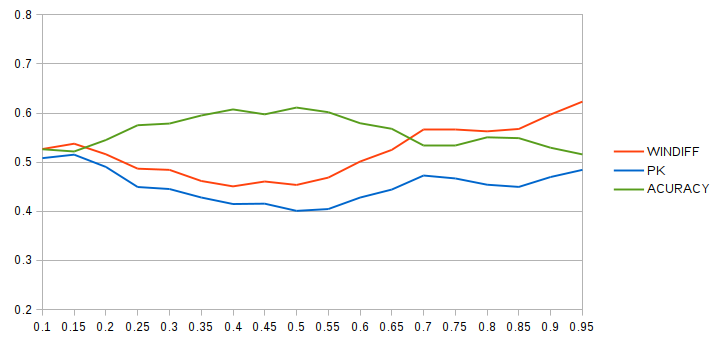
\includegraphics[width=1\textwidth]{conteudo/capitulos/figs/graficos/analiseNSegRate-MinCut.png}
	  \caption{Performance dos algoritmos de segmentação textual}
	  \label{fig:grafico-medidas-tradicionais}
  \end{figure}


  \begin{figure}[!h]
	  \centering
	  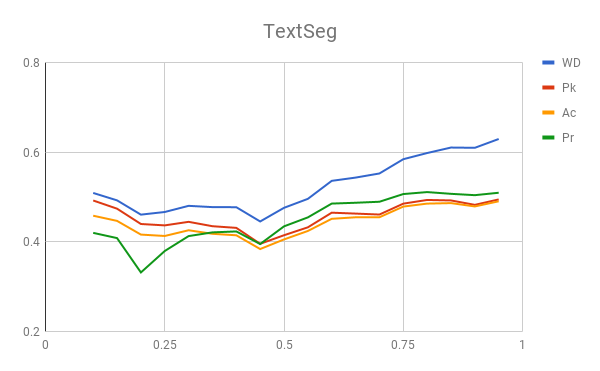
\includegraphics[width=1\textwidth]{conteudo/capitulos/figs/graficos/analiseNSegRate-UISeg.png}
	  \caption{Performance dos algoritmos de segmentação textual}
	  \label{fig:grafico-medidas-tradicionais}
  \end{figure}

  \begin{figure}[!h]
	  \centering
	  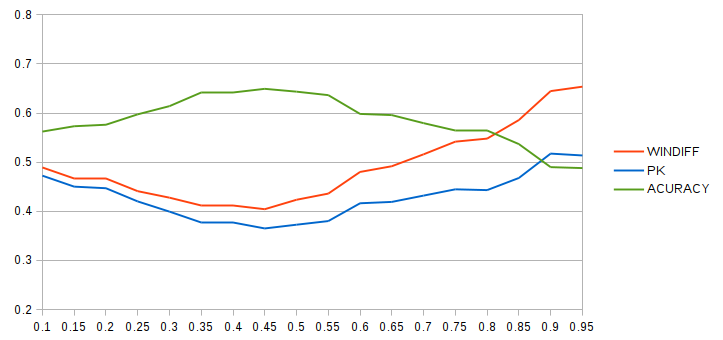
\includegraphics[width=1\textwidth]{conteudo/capitulos/figs/graficos/analiseNSegRate-Bayes.png}
	  \caption{Performance dos algoritmos de segmentação textual}
	  \label{fig:grafico-medidas-tradicionais}
  \end{figure}

  
  \begin{figure}[!h]
	  \centering
	  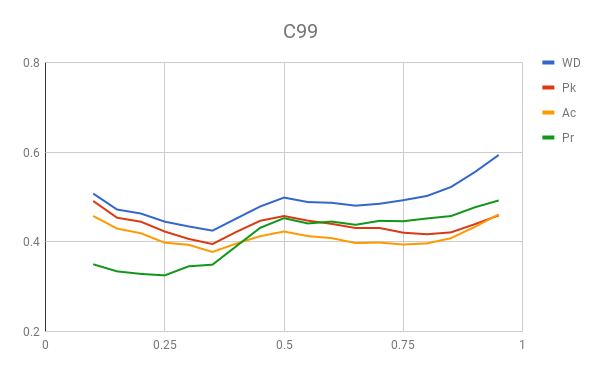
\includegraphics[width=1\textwidth]{conteudo/capitulos/figs/graficos/analiseNSegRate-C99.png}
	  \caption{Performance dos algoritmos de segmentação textual}
	  \label{fig:grafico-medidas-tradicionais}
  \end{figure}


  
  \begin{figure}[!h]
	  \centering
	  \includegraphics[width=1\textwidth]{}
	  \caption{Performance dos algoritmos de segmentação textual}
	  \label{fig:grafico-medidas-tradicionais}
  \end{figure}



% ------------------------------



\begin{table}[!h]
	\centering
	\begin{tabular}{|l||c|c|c|c|c|c|c|c|c|c|c|} \hline

		\textbf{Algoritmo} && 
		\textbf{Step} &
		\textbf{Win} & 
		\textbf{P$_k$} & 
		\textbf{WD} & 
		\textbf{Ac} & 
		\textbf{Pr} & 
		\textbf{Re} &
		\textbf{F$^1$} &
		\textbf{\#Segs} \\	\hline

TextTiling && 20 & 30 & 0.461 & 0.444 & 0.581 & 0.560 & \cellcolor{gray!20} \textbf{0.336} & \cellcolor{gray!20} \textbf{0.411} & 8.833  \\ \hline 
TextTiling && 30 & 45 & \cellcolor{gray!20} \textbf{0.450} & \cellcolor{gray!20} \textbf{0.435} & \cellcolor{gray!20} \textbf{0.596} & \cellcolor{gray!20} \textbf{0.696} & 0.275 & 0.373 & 6.417  \\ \hline 

\hline
		\textbf{Algoritmo} &
		\textbf{RS} &
		\textbf{W} & 
		\textbf{SRate}& 
		\textbf{P$_k$} & 
		\textbf{WD} & 
		\textbf{Ac} & 
		\textbf{Pr} & 
		\textbf{Re} &
		\textbf{F$^1$} &
		\textbf{\#Segs} \\	\hline

C99 & 3 & true  &0.300 &  \cellcolor{gray!20} \textbf{0.434} & \cellcolor{gray!20} \textbf{0.407} & 0.607 & 0.655 & 0.376 & 0.457 & 9.250  \\ \hline 
C99 & 3 & true  &0.700 &  0.485 & 0.431 & 0.602 & 0.553 & \cellcolor{gray!20} \textbf{0.797} & \cellcolor{gray!20} \textbf{0.633} & 21.417  \\ \hline 
C99 & 5 & true  &0.500 &  0.460 & 0.421 & \cellcolor{gray!20} \textbf{0.609} & 0.580 & 0.600 & 0.571 & 15.500  \\ \hline 
C99 & 3 & false &0.200 &  0.448 & 0.427 & 0.596 & \cellcolor{gray!20} \textbf{0.719} & 0.257 & 0.362 & 6.083  \\ \hline 


\hline
		\textbf{Algoritmo} && 
		\textbf{Cut} & 
		\textbf{SRate} &
		\textbf{P$_k$} & 
		\textbf{WD} & 
		\textbf{Ac} & 
		\textbf{Pr} & 
		\textbf{Re} &
		\textbf{F$^1$} &
		\textbf{\#Segs} \\	\hline


MinCutSeg && 13 & 0.300 & 0.457 & 0.427 & 0.594 & \cellcolor{gray!20} \textbf{0.638} & 0.353 & 0.433 & 8.667  \\ \hline 
MinCutSeg && 9  & 0.400 & \cellcolor{gray!20} \textbf{0.444} & 0.408 & \cellcolor{gray!20} \textbf{0.614} & 0.629 & 0.494 & 0.526 & 11.917  \\ \hline 
MinCutSeg && 11 & 0.500 & 0.459 & \cellcolor{gray!20} \textbf{0.407} & 0.603 & 0.588 & 0.590 & 0.563 & 15.000  \\ \hline 
MinCutSeg && 5  & 0.700 & 0.528 & 0.438 & 0.567 & 0.536 & \cellcolor{gray!20} \textbf{0.746} & \cellcolor{gray!20} \textbf{0.599} & 21.000  \\ \hline 


\hline
		\textbf{Algoritmo} &
		\textbf{Prior} &
		\textbf{Disp.} & 
		\textbf{SRate}& 
		\textbf{P$_k$} & 
		\textbf{WD} & 
		\textbf{Ac} & 
		\textbf{Pr} & 
		\textbf{Re} &
		\textbf{F$^1$} &
		\textbf{\#Segs} \\	\hline


 BayesSeg & 0.0800 & 0.5000 &  Auto & \cellcolor{gray!20} \textbf{0.380} & \cellcolor{gray!20} \textbf{0.361} & \cellcolor{gray!20} \textbf{0.655} & 0.662 & 0.479 & 0.551 & 10.000  \\ \hline 
 BayesSeg & 0.1100 & 0.5000 &  Auto & 0.388 & 0.370 & 0.649 & \cellcolor{gray!20} \textbf{0.672} & 0.433 & 0.523 & 9.000  \\ \hline 
 BayesSeg & 0.1100 & 0.1000 & 0.600 & 0.462 & 0.399 & 0.615 & 0.574 & 0.724 & \cellcolor{gray!20} \textbf{0.619} & 18.417  \\ \hline 
 BayesSeg & 0.0800 & 0.1000 & 0.900 & 0.645 & 0.517 & 0.490 & 0.478 & \cellcolor{gray!20} \textbf{0.878} & 0.600 & 27.500  \\ \hline 

\hline
		\textbf{Algoritmo} &&&
		\textbf{SRate} & 
		\textbf{P$_k$} & 
		\textbf{WD} & 
		\textbf{Ac} & 
		\textbf{Pr} & 
		\textbf{Re} &
		\textbf{F$^1$} &
		\textbf{\#Segs} \\	\hline

TextSeg &&& Auto & \cellcolor{gray!20} \textbf{0.455} & 0.439 & 0.585 & \cellcolor{gray!20} \textbf{0.618} & 0.266 & 0.368 & 6.417  \\ \hline 
TextSeg &&& 0.500 & 0.475 & \cellcolor{gray!20} \textbf{0.417} & \cellcolor{gray!20} \textbf{0.594} & 0.565 & 0.608 & 0.566 & 15.500  \\ \hline 
TextSeg &&& 0.900 & 0.604 & 0.484 & 0.524 & 0.498 & \cellcolor{gray!20} \textbf{0.922} & \cellcolor{gray!20} \textbf{0.627} & 27.500  \\ \hline 

\hline
		\textbf{Algoritmo} &&&
		\textbf{SRate} & 
		\textbf{P$_k$} & 
		\textbf{WD} & 
		\textbf{Ac} & 
		\textbf{Pr} & 
		\textbf{Re} &
		\textbf{F$^1$} &
		\textbf{\#Segs} \\	\hline


Sentenças &&& 1.000& \cellcolor{gray!20} \textbf{0.640} & \cellcolor{gray!20} \textbf{0.490} & \cellcolor{gray!20} \textbf{0.506} & \cellcolor{gray!20} \textbf{0.488} & \cellcolor{gray!20} \textbf{1.000} & \cellcolor{gray!20} \textbf{0.638} & 30.500  \\ \hline 



	\end{tabular}
	\caption{Resultados obtidos com o \textit{TextTiling}}
	\label{tab:resultadosTT}
\end{table}




% Katti, Removi o texto que estava a seguir, junto com os gráficos que já conversamos. Estou escrevendo ainda essa parte. Daqui em diante pretendo: Discutir melhor esses gráficos conforme conversamos. Discutir a influência quantidade de segmentos. Incluir os resultados do último experimento.






% \begin{table}[!h]
	% \centering
% \begin{tabular}{|l||c|c|c|c|c|c|c|} 
% \hline 
% \textbf{M\'{e}todo} & 
% \textbf{Pk} & 
% \textbf{WD} & 
% \textbf{A } & 
% \textbf{P } & 
% \textbf{R } & 
% \textbf{F1} & 
% \textbf{Segmentos}\\ \hline

% Senten\c{c}as & 0.320 & 0.502 & 0.498 & 0.498 & \textbf{1.000} & \textbf{0.642} & 22.083\\ \hline
% TextTiling    & 0.275 & 0.469 & 0.531 & 0.514 & 0.937 & 0.640 & 19.583\\ \hline
% C99           & 0.142 & 0.426 & 0.574 & 0.601 & 0.473 & 0.506 & 8.167\\ \hline
% BayesSeg      & 0.148 & 0.414 & 0.586 & 0.599 & 0.526 & 0.528 & 8.750\\ \hline
% MinCut        & 0.226 & 0.532 & 0.468 & 0.464 & 0.438 & 0.432 & 10.333\\ \hline
% TextSeg       & \textbf{0.085} & \textbf{0.387} & \textbf{0.613} & \textbf{0.714} & 0.412 & 0.497 & 5.167\\ \hline
% \end{tabular} 

	% \caption{Melhores resultados obtidos.}
	% \label{tab:configfinal}
% \end{table}




%--> TODO: explicar (a conceituação teórica) que passos curtos geram mais segmentos

  % \begin{figure}[!h]
	  % \centering
	  % 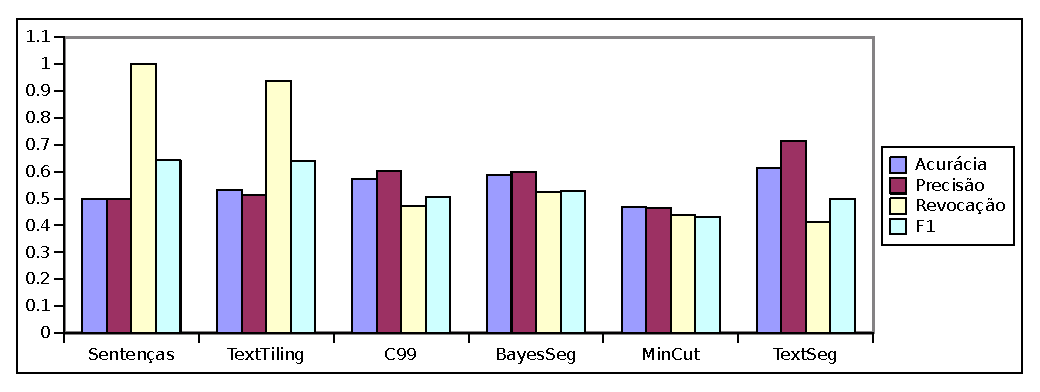
\includegraphics[width=1\textwidth]{conteudo/capitulos/figs/grafico-medidas-APRF1.eps}
	  % \caption{Performance dos algoritmos de segmentação textual com as medidas tradicionais}
	  % \label{fig:grafico-medidas-tradicionais}
  % \end{figure}
  

% Na Figura~\ref{fig:grafico-medidas-Pk-Wd} é apresentada a performance dos algoritmos nas medidas P$_k$ e \textit{WindowDiff}. Verifica-se que \textit{TextSeg} apresenta valores de \textit{WindowDiff} próximas ao \textit{C99} e \textit{BayesSeg} e resultados mais significantes quando medidos por P$_k$ em relação aos demais algoritmos.



  % \begin{figure}[!h]
	  % \centering
	  % 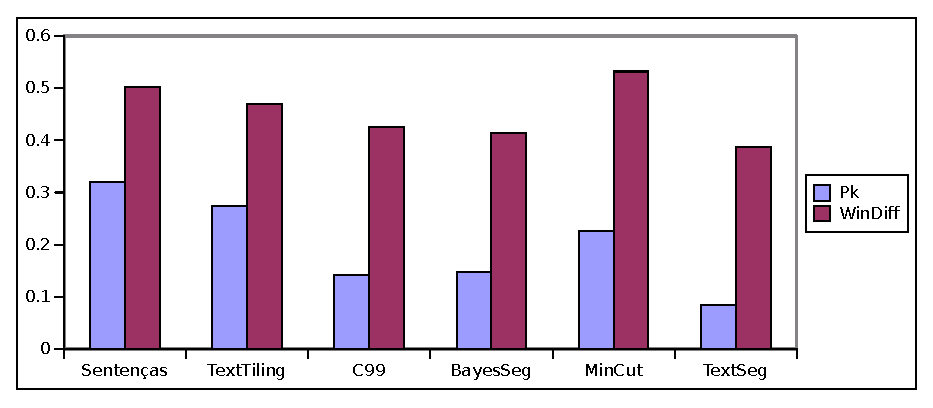
\includegraphics[width=1\textwidth]{conteudo/capitulos/figs/grafico-medidas-Pk-Wd.eps}
	  % \caption{Performance dos algoritmos de segmentação textual com as medidas P$_k$ e \textit{WindowDiff}.}
	  % \label{fig:grafico-medidas-Pk-Wd}
  % \end{figure}




  % \begin{figure}[!h]
	  % \centering
	  % 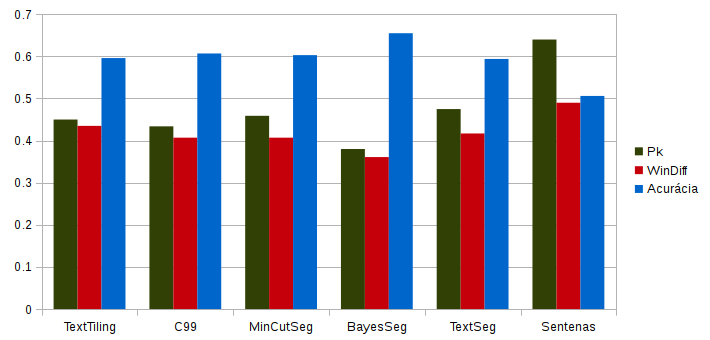
\includegraphics[width=1\textwidth]{conteudo/capitulos/figs/graficos/resumo-5.png}
	  % \caption{Performance dos algoritmos de segmentação textual}
	  % \label{fig:grafico-medidas-tradicionais}
  % \end{figure}






% -? Medidas
% -- como ele faz?



% Outro ponto a ser analisado é a influência da proporção de segmentos identificados na performance do algoritmo. Durante os testes observou-se que os parâmetros relacionados a quantidade de segmentos causam maior impacto nas medidas de desempenho. Na Figura~\ref{fig:influencia-SegRate} é exibida a relação entre a taxa de segmentação e as medidas de desempenho as quais apresentam melhores valores entre $30\%$ e $50\%$ de sentenças marcadas como final de segmento.



% \begin{figure}[!h] \centering     %%% not \center

	% \subfigure{ \label{fig:influencia-segRate-c99}
	  % 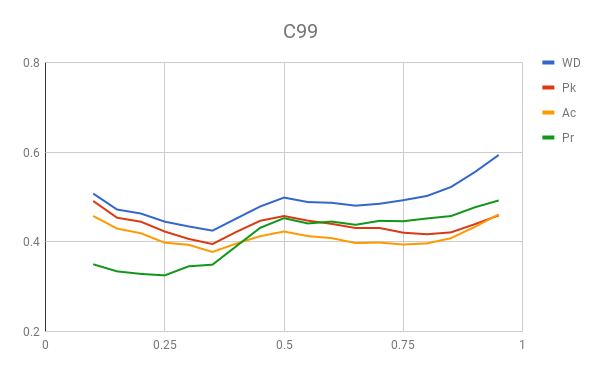
\includegraphics[width=.48\textwidth]{conteudo/capitulos/figs/graficos/analiseNSegRate-C99.png}
	% }
	% \subfigure{ \label{fig:influencia-segRate-mc}
	  % 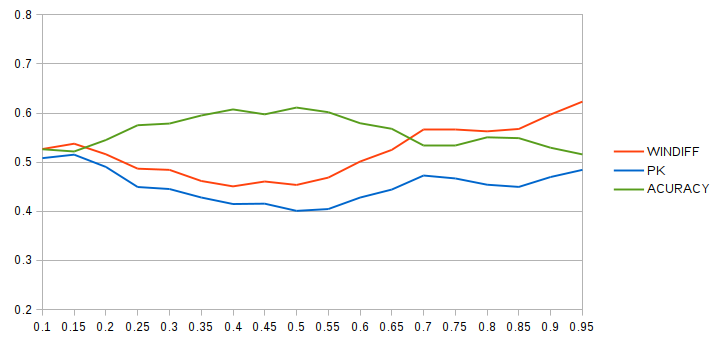
\includegraphics[width=.48\textwidth]{conteudo/capitulos/figs/graficos/analiseNSegRate-MinCut.png}
	% }
	% \subfigure{ \label{fig:influencia-segRate-bs}
	  % 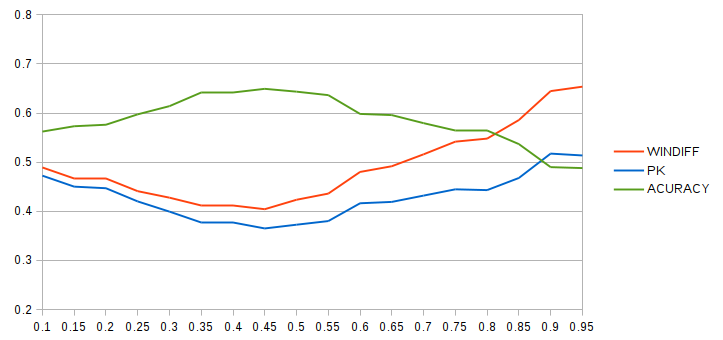
\includegraphics[width=.48\textwidth]{conteudo/capitulos/figs/graficos/analiseNSegRate-Bayes.png}
	% }
	% \subfigure{ \label{fig:influencia-segRate-ui}
	  % 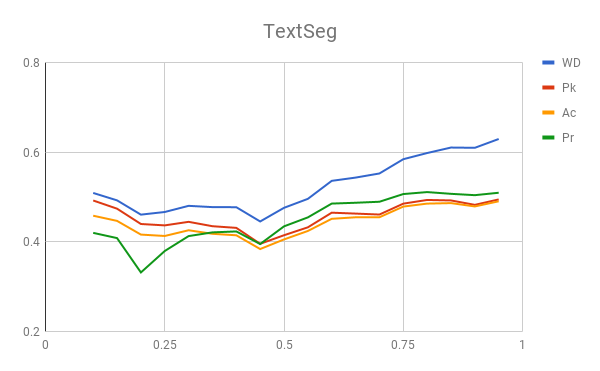
\includegraphics[width=.48\textwidth]{conteudo/capitulos/figs/graficos/analiseNSegRate-UISeg.png}
	% }
	% \caption{Influência do taxa segmentos na eficiência dos algoritmos}
	% \label{fig:influencia-SegRate}
% \end{figure}






Ata      ; Sent. ;  A1  ;   A2 ;  A3 ;  A4 ;   A5 ;   A6 ;   A7 ;   A8 ;   A9  ;  k      ;  P k   ;   WD
Ata 1    ; 25    ;  7   ;   4  ;  11 ;  6  ;   16 ;   8  ;   8  ;   15 ;   16  ;  0.344  ;  0.593 ;   0.475
Ata 2    ; 17    ;  4   ;   4  ;  8  ;  6  ;   11 ;   6  ;   6  ;   15 ;   14  ;  0.377  ;  0.572 ;   0.509
Ata 3    ; 26    ;  6   ;   6  ;  8  ;  4  ;   15 ;   9  ;   10 ;   18 ;   14  ;  0.384  ;  0.603 ;   0.524
Ata 4    ; 26    ;  5   ;   5  ;  10 ;  6  ;   14 ;   17 ;   7  ;   11 ;   12  ;  0.447  ;  0.652 ;   0.540
Ata 5    ; 33    ;  4   ;   4  ;  6  ;  5  ;   17 ;   22 ;   9  ;   18 ;   16  ;  0.315  ;  0.595 ;   0.364
Ata 6    ; 11    ;  3   ;   4  ;  6  ;  4  ;   9  ;   9  ;   4  ;   7  ;   5   ;  0.397  ;  0.605 ;   0.576
Ata 7    ; 20    ;  3   ;   7  ;  5  ;  4  ;   11 ;   14 ;   5  ;   5  ;   4   ;  0.374  ;  0.658 ;   0.506
Ata 8    ; 35    ;  4   ;   8  ;  3  ;  8  ;   12 ;   17 ;   5  ;   11 ;   9   ;  0.378  ;  0.611 ;   0.471
Ata 9    ; 24    ;  3   ;   5  ;  3  ;  6  ;   11 ;   11 ;   3  ;   9  ;   9   ;  0.428  ;  0.591 ;   0.478
Ata 10   ; 50    ;  4   ;   5  ;  4  ;  7  ;   31 ;   29 ;   5  ;   9  ;   8   ;  0.309  ;  0.598 ;   0.233
Ata 11   ; 43    ;  4   ;   7  ;  5  ;  7  ;   29 ;   19 ;   5  ;   9  ;   12  ;  0.348  ;  0.645 ;   0.412
Ata 12   ; 56    ;  3   ;   10 ;  4  ;  16 ;   33 ;   25 ;   4  ;   13 ;   11  ;  0.278  ;  0.577 ;   0.102




% \begin{table}[!h]
	% \centering
	% \begin{tabular}{|l||c|c|c||c|c|c|} \hline

		% & \multicolumn{3}{c||}{Sem Pré-processamento} 
		% & \multicolumn{3}{c|}{Com Pré-processamento}\\			

		% \textbf{Medida} & 
		% \textbf{J} &
		% \textbf{P} & 
		% \textbf{Média} &
		% \textbf{J} &
		% \textbf{P} & 
		% \textbf{Média} \\	\hline

		% P$_k$				& 50 & 9 & 0,142 & 50 & 9  & 0,144 \\ \hline
		% \textit{WindowDiff}	& 50 & 6 & 0,387 & 40 & 9  & 0,396 \\ \hline
		% Acurácia			& 50 & 6 & 0,612 & 40 & 9  & 0,603 \\ \hline
		% Precisão			& 40 & 9 & 0,611 & 50 & 12 & 0,613 \\ \hline
		% Revocação			& 20 & 3 & 0,886 & 20 & 3  & 0,917 \\ \hline
		% F$^1$				& 30 & 6 & 0,605 & 40 & 3  & 0,648 \\ \hline

	% \end{tabular}
	% \caption{Resultados obtidos com o \textit{TextTiling}}
	% \label{tab:resultadosTT}
% \end{table}











% \begin{table}[!h]
	% \centering
	% \begin{tabular}{|l||c|c|c|c||c|c|c|c|} \hline

		% & \multicolumn{4}{c||}{Sem Pré-processamento} 
		% & \multicolumn{4}{c|}{Com Pré-processamento}\\			

		% \textbf{Medida} & 
		% \textbf{S} & 
		% \textbf{M} & 
		% \textbf{W} & 
		% \textbf{Média} &
		% \textbf{S} & 
		% \textbf{M} & 
		% \textbf{W} & 
		% \textbf{Média} \\	\hline

		% P$_k$				& 20 & 9 & Sim & 0,134& 20 & 11 & False	& 0,116 \\ \hline  
		% \textit{WindowDiff}	& 60 & 9 & Sim & 0,411& 60 &  9 & Sim 	& 0,390 \\ \hline  
		% Acurácia			& 60 & 9 & Sim & 0,588& 60 &  9 & Sim 	& 0,609 \\ \hline  
		% Precisão			& 40 & 9 & Sim & 0,645& 20 & 11 & False	& 0,720 \\ \hline  
		% Revocação			& 80 & 9 & Sim & 0,869& 80 & 11 & Sim 	& 0,897 \\ \hline  
		% F$^1$				& 80 & 9 & Sim & 0,638& 80 & 11 & Sim 	& 0,655 \\ \hline  

	% \end{tabular}
	% \caption{Resultados obtidos com o \textit{C99}}
	% \label{tab:resultadosc99}
% \end{table}




% Concluído o processo, os dados foram reunidos e tratados para que todo segmento termine em um final de sentença. Uma vez que software dava o anotador liberdade para segmentar o texto após qualquer character do texto, os finais de segmento movidos para que o resultado se adequasse ao formato dos algoritmos segmentação em que usa-se sentenças como unidade básica de informação, conforme já mencionado no Algoritmo~\ref{alg:identificacaofinaisdesent}. A Tabela~\ref{tab:ataseanotacoes}, mostra para cada ata a quantidade de sentenças e segmentos identificados pelos anotadores.




% os dados foram reunidos e gerou-se um conjunto de 12 atas segmentadas manualmente por 9 anotadores, totalizando 108 anotações. A Tabela~\ref{tab:ataseanotacoes}, mostra para cada ata a quantidade de sentenças e segmentos identificados pelos anotadores.



% Nesse trabalho, para cada segmentação fornecida por cada anotador calcula-se as medidas \textit{WindowDiff}, $P_k$ e \textit{Kappa}.







\begin{table}[!h]
	\centering
 \begin{tabular}{|c|c|c|c|c|}

\hline
\textbf{Referência}  & \textbf{\#Seg} & \textbf{\textit{Kappa}}       & \textbf{\textit{P}$_k$}                &  \textbf{\textit{WinDiff}}\\ \hline
Ref. 01     & 15    & 0,344  $\sigma$0,190 & 0,433  $\sigma$0,170 & 0,631  $\sigma$0,409 \\ \hline
Ref. 02     & 13    & 0,266  $\sigma$0,246 & 0,439  $\sigma$0,190 & 0,565  $\sigma$0,379 \\ \hline
Ref. 03     & 15    & 0,328  $\sigma$0,183 & 0,442  $\sigma$0,165 & 0,590  $\sigma$0,353 \\ \hline
Ref. 04     & 15    & 0,364  $\sigma$0,241 & 0,364  $\sigma$0,161 & 0,562  $\sigma$0,377 \\ \hline
Ref. 05     & 19    & 0,315  $\sigma$0,217 & 0,458  $\sigma$0,223 & 0,889  $\sigma$0,640 \\ \hline
Ref. 06     & 9     & 0,314  $\sigma$0,218 & 0,404  $\sigma$0,163 & 0,463  $\sigma$0,266 \\ \hline
Ref. 07     & 8     & 0,235  $\sigma$0,208 & 0,343  $\sigma$0,192 & 0,507  $\sigma$0,401 \\ \hline
Ref. 08     & 12    & 0,211  $\sigma$0,225 & 0,421  $\sigma$0,186 & 0,629  $\sigma$0,479 \\ \hline
Ref. 09     & 12    & 0,234  $\sigma$0,258 & 0,472  $\sigma$0,203 & 0,660  $\sigma$0,427 \\ \hline
Ref. 10     & 13    & 0,170  $\sigma$0,206 & 0,428  $\sigma$0,227 & 0,937  $\sigma$1,050 \\ \hline
Ref. 11     & 12    & 0,209  $\sigma$0,236 & 0,368  $\sigma$0,203 & 0,704  $\sigma$0,654 \\ \hline
Ref. 12     & 21    & 0,222  $\sigma$0,195 & 0,452  $\sigma$0,200 & 0,113  $\sigma$1,202 \\ \hline
\textbf{Total}      & \textbf{13.666} & \textbf{0,267}  \textbf{$\sigma$0,218} & \textbf{0,418}  \textbf{$\sigma$0,190} & \textbf{0,604}  \textbf{$\sigma$0,553} \\ \hline
\end{tabular}
\caption{Medidas de concordância entre os anotadores sobre cada ata segmentada manualmente.}
\label{tab:detalhesSegRef}
\end{table}





% Os algoritmos \textit{TextTiling} e \textit{C99} são analisados devido a sua abordagem linguística baseada em coesão léxica e por estarem entre os primeiros trabalhos nessa área e serem frequentemente referenciados até hoje~\cite{AlemiG15}. 









O trabalho de rotulação do assunto de cada seguimento, constituiu-se em 3 passos:
(1) classificação quanto ao tipo de comunicação, onde se especificou uma entre as opções 
\textit{``decisão``},
\textit{``informe''} e 
\textit{``irrelevante''}. 
% e \textit{``outro''} sendo que para essa última, o anotador poderia especificar livremente a classe.
(2) classificação quanto ao ao contexto onde se gerou o assunto, onde as classes, 
\textit{``discussão''},
\textit{``orientação''} e	
\textit{``solicitação''} podendo o anotador indicá-las simultaneamente.
% \textit{``outro''} podendo o anotador indicá-las simultaneamente.
Para os passos 1 e 2 havia a opção \textit{``outro''} em que o anotador poderia especificar livremente o tipo e o contexto do assunto.
(3) descrição do assunto, onde o anotador apontou até 5 palavras contidas no texto para representar o teor do segmento.
Esses rótulos tem como propósito ajudar a descrever os segmentos de atas por meio de classes e descritores, podendo ser utilizados na etapa de treinamento de classificadores e avaliação de extratores de tópicos.
Na Figura~\ref{fig:interfaceanotacoes} é mostrada a interface da ferramenta utilizada para as anotações.




